\documentclass[usenatbib,fleqn]{mn2e}
\usepackage{amsmath,amssymb}
\usepackage{graphicx}
\usepackage{epstopdf}
\epstopdfsetup{outdir=./figures/}
\graphicspath{{./figures/}}
\usepackage{url}
\usepackage{aas_macros}
\usepackage{astro}
\usepackage{natbib}


\newcommand{\eddr}{\dot{M}/\dot{M}_{\rm Edd}}
\newcommand{\Mdotb}{\dot{M}_{\rm bondi}}

\newcommand\lsim{\mathrel{\rlap{\lower4pt\hbox{\hskip1pt$\sim$}}
        \raise1pt\hbox{$<$}}}
\newcommand\gsim{\mathrel{\rlap{\lower4pt\hbox{\hskip1pt$\sim$}}
        \raise1pt\hbox{$>$}}}
\newcommand{\rs}{r_s}
\newcommand{\rb}{r_b}
\newcommand{\vw}{v_w}
\newcommand{\cs}{c_s}

\newcommand{\dxdy}[2]{\frac{\partial #1}{\partial #2} }
\newcommand{\ddr}[1]{\dxdy{#1}{r}}
\newcommand{\drhodt}{\dxdy{\rho}{t}}
\newcommand{\dpdr}{\dxdy{p}{r}}
\newcommand{\dvdr}{\dxdy{v}{r}}
\newcommand{\dsdr}{\dxdy{s}{r}}
\newcommand{\dphidr}{\dxdy{\Phi}{r}}
\newcommand{\ke}{\frac{v^2}{2}}
\newcommand{\kew}{\frac{v_w^2}{2}}
\newcommand{\gammaf}{\frac{\gamma}{\gamma-1}}
\newcommand{\gammafi}{\frac{\gamma-1}{\gamma}}
\newcommand{\cs}{\frac{p}{\rho}}
\newcommand{\Q}{q (\ke+\kew-\gammaf \cs)}
\newcommand{\kb}{k_{\rm b}}
\renewcommand{\mp}{m_{\rm p}}
\newcommand{\Menc}{M_{\rm enc}}
\newcommand{\Mstar}{M_{*}}
\newcommand{\Mbh}[1][]{M_{\bullet#1}}
\newcommand{\phirs}{\frac{G \Menc}{\rs}}
\newcommand{\soi}{\rm soi}
\newcommand{\ff}{\rm ff}
\newcommand{\rsoi}{r_{\soi}}
\newcommand{\sigsoi}{\sigma_{\soi}}
\newcommand{\vwO}{v_{w,0}}
\newcommand{\x}{\frac{r_s}{\rsoi}}
\newcommand{\vwNorm}{\frac{\vwO}{\sigsoi}}
\newcommand{\pyear}{{\rm yr}^{-1}}

\topmargin -1 cm
\defcitealias{WangMerritt:2004a}{WM04}	

\author[Generozov, Metzger, \& Stone]{Aleksey Generozov$\thanks{E-mail: ag@astro.columbia.edu}$, Nicholas Stone, Brian~D.~Metzger$\footnotemark[1]$\\
Columbia Astropysics Labratory, Columbia University, 550 West 120th Street, New York, NY 10027}


\begin{document}
\title{Constraining Supermassive Black Hole Environments.}
 \maketitle

\begin{abstract}
Abstract here 
\end{abstract}

 \begin{keywords}
 black hole physics --  galaxies: active
 \end{keywords}


\section{Introduction}
\label{sec:introduction}

%%Maybe active galaxies constitute 10% need reference here?
Supermassive black holes (SMBHs) are present in the centers of most,
if not all nearby galaxies (see reviews by, e.g. \citealt{KormendyRichstone:1995a};
\citealt{FerrareseFord:2005a}). Roughly $\sim 1\%$ of these manifest themselves as luminous Active Galactic Nuclei. However, quiescent black holes constitute a silent majority. 

In order to understand why most galaxies appear to be inactive, it is necessary to understand the gas environment of black holes, as the gas density around the black hole sets its accretion rate.  The accretion rate in turn has implications for rate of black hole growth. 

The gas environment also plays an important role in determining observables (light-curves, SEDs) from jetted tidal disruption events (TDEs). These are bright flares that occur when a star passes within the tidal disruption radius of the SMBH. A small fraction of such events are accompanied by the launch of a relativistic jet into the circumnuclear medium (CNM) of the host galaxy.  As the jet propagates into the CNM, a reverse shock propagates towards the back of the jet, decelerating it. The CNM density profile will determine the final Lorentz factor of the jet. This in turn will strongly affect the duration of the observed synchotron radiation. 

The gas in the vicinity of a black hole may come from several sources. \citealt{Ho:2009a} proposes three different mechanisms (1) Mass loss in winds (particularly from evolved stars) (2) Stellar-stellar collisions in dense environments (3) Tidal disruptions of stars. To estimate (a lower limit on the accretion rate), \citealt{Ho:2009a} calculates the Bondi accretion rate based on typical observed gas densities and temperatures taken from Chandra X-ray observations. A second estimate is obtained from the wind mass loss rate from the observed stellar densities. Both of the estimates suggest that there is an ample reservoir of gas to power active galactic nuclei in quiescent galaxies. This suggests that the lack of the AGN activity is due to the fact that the the accretion proceeds in a radiatively inefficient mode. 

Previous studies used Chandra observations to show that the Bondi accretion power well-correlated with jet power \citep{AllenDunn+:2006a,Fujita+:2013a}. In these studies temperature, and density information are inferred from Chandra x-ray observations, while the jet power is inferred from the energy required to inflate observed bubbles within the x-ray emitting gas. 

However, this approach has limitations. Due to resolution issues it is almost never possible to observationally determine the gas density at the black sphere of influence, and such studies are forced to extrapolate observed gas temperatures and densities to smaller scales.  In fact, the temperature profile is assumed to be flat inside of the Bondi radius.  In reality, the cusp in the velocity dispersion near the SMBH, should cause a cusp in the gas temperature profile (assuming the kinetic energy of stellar winds is efficiently themalized in shocks). 
%%AG-give sense of scale.

Another approach to constraining the gas density around an SMBH is to go from a stellar mass loss rate (motivated by observed stellar densities) to a steady-state gas profile. This approach was taken by \citealt{Quataert:2004a,De-ColleGuillochon+:2012a,ShcherbakovWong+:2014a}. 

%In this study we perform hydrodynamic modeling to solve for the steady-state gas density, temperature and velocity profiles near the SMBH sphere of influence, for a sample of nearby, quiescent galaxies. We a adopt the model used by \cite{Quataert:2004a} for the galactic center: gas is supplied by stellar winds, which collide, shock heat, and thermalize.  
We take the same approach. To the best of our knowledge a systematic study of the parameter space of central galaxy properties. Thus, we compute central density profiles for a broad sample of galaxies for \cite{WangMerritt:2004a}--henceforward \citetalias{WangMerritt:2004a}.  This allows us to determine to relate the central stellar properties (e.g. stellar density slope) to the central gas properties. 

We also explore the effects of varying the heating rate on the flow structure. Typically an inflow outflow flow structure is established. The stellar ejecta inside of the stagnation radius ($\rs$) will be accreted, while that outside $\rs$ will be driven out with the outflow. The location of $\rs$ and hence the accretion rate is  quite sensitive to the assumed heating rate.  In fact, as the specific thermal energy of the ejects drops below the potential, an inflow is established out to the radius where the SNe Ia rate becomes comparable to the dynamical timescale, which for black holes smaller than 10$^8 \Msun$ is well outside the $\rsoi$ 
%It turns out that in our models the mass accretion rate is coincidentally quite similar to the Bondi accretion rate.

 %%AG--say something about x-ray observations. 


\section{Sample}
Describe WM/Nuker sample here.

\section{Model}
We use the same model as \citealt{Quataert:2004a} to find a steady state gas density near the SMBH for each of the galaxies within our sample.  Gas is supplied by winds from the stellar population in the galactic center. Assuming a rate of mass injection, $q$, spherical symmetry and an ideal gas equation of state. 

\begin{align}
&\drhodt+\frac{1}{r^2}\dxdy{\rho r^2 v}{r}=q\\
&\rho \frac{dv}{dt}=-\dpdr-\rho \dphidr-q v\\
&\rho T \frac{ds}{dt}=q\left[\ke+\kew+\gammaf \cs \right]
\end{align}

These or similar equations have been solve many times in the literature (e.g. \citealt{HolzerAxelford1971a,Quataert:2004a,De-ColleGuillochon+:2012a,ShcherbakovWong+:2014a}). \citealt{ShcherbakovWong+:2014a} solves similar equation, with additional terms to account for thermal conduction and radiative cooling. However, we find that radiative cooling may be neglected for a large portion of our parameter space--\S~\ref{sec:cooling}.  Additionally thermal conduction may be cut off by magnetic field lines--\S~\ref{sec:conduction}

$q$ represent the rate of injection of gas mass per unit volume, and is derived from the stellar density, $\rho_*$, using

\begin{align}
q=\frac{\eta \rho_*}{t_h}
\end{align}

%%AG $eta/th$ is the specific of rate of mass return to the ISM.  Ciotti et al. 1991 -- see in particular Table 2. 
Where $t_h$ is the Hubble time, and $\eta$ is an efficiency parameter--for a stellar population between 2-15 Gyr old, this 
number will lie in the range $\sim$0.1-1. We adopt $\eta=1$. However, scaling $\eta$ by some factor, would simply scale the $\rho$ by the same factor and otherwise leave the solution unchanged.

$v_w^2/2$ encapsulates heating in our simulation. We take $v_w^2=\sqrt{\sigma(r)^2+v_{w,0}^2}$ where $\sigma(r)$ corresponds to the velocity dispersion of the stars and $v_{w,0}$ accounts for additional heating sources (ms pulsars, SNe Ia, etc.)  We approximate $\sigma(r)$ to be given by $G \Menc/r=G(\Mbh+\Mstar)/r$, where $\Mbh$ is the mass of the SMBH and $\Mstar$ is the stellar mass inside radius $r$. 

\section{Solutions}
\subsection{Analytics: Location of Stagnation Radius}
It is possible to derive an analytic expression for the steady-state stagnation radius, $\rs$, in terms of $v_w$ and the power law slope of the density at $\rs$.

Consider the steady-state entropy equation.

\begin{align}
&\rho T v \dsdr=\Q\\
&\dsdr=\frac{\Q}{\rho T v} \label{eq:ss_entropy}
\end{align}

At $\rs$, the velocity, $v$ goes to zero.  Therefore, the numerator must also go to 0 at $\rs$. This implies 

\begin{align}
 &\kew-\gammaf \cs=0\\
 &\cs=\gammafi \kew\\
 &\frac{\kb T}{\mu \mp}=\gammafi \kew \label{eq:tstag}
\end{align}

From the first law of thermodynamics 

\begin{align}
T\dsdr&=\ddr{u}+p\ddr{(1/\rho)}\\
&=\frac{1}{\gamma-1}\ddr{(p/\rho)}-\frac{p}{\rho^2}\ddr{\rho}\\
&=\frac{1}{\gamma-1}\ddr{(p/\rho)}-\frac{p}{\rho} \underbrace{\dxdy{\log{\rho}}{\log{r}}}_{-n} \label{eq:first_law}
\end{align}

Combining Equation~\ref{eq:first_law} and Equation~\ref{eq:ss_entropy}, one obtains.

\begin{align}
\frac{1}{\gamma-1}\ddr{(p/\rho)}+r n \cs=\frac{\Q}{\rho  v} \label{eqn:combo1}
\end{align}

At the stagnation point we also have (from the momentum equation)

\begin{align}
&\frac{1}{\rho}\dpdr=-\dphidr\\
&\ddr{(p/\rho)}-r n \cs=-\dphidr \label{eqn:HSE}
\end{align}

Then multiplying Equation~\ref{eqn:HSE}  $\frac{1}{\gamma-1}$ and subtracting it from Equation~\ref{eqn:combo1} we obtain

\begin{align}
\gammaf r n \cs = \frac{1}{\gamma-1} \dphidr + \frac{\Q}{\rho  v}
\end{align}

From the above equation we may obtain an expression for the Stagnation point using L'Hopital's rule and Equation~\ref{eq:tstag}. To obtain an analytic expression, we take $\Mstar\sim r^{2-\Gamma}$

\begin{align}
&\kew n =A \phirs -B \frac{G \Mbh}{\rs}\\
&A=\left[\frac{4\gamma-(\gamma-1)(1+\Gamma)}{4(\gamma-1)}\right]; \hspace{1cm} B=\frac{2-\Gamma}{4} \label{eq:stag_analytic}
\end{align}

Note that in the above expression $\Mstar$ is evaluated at the stagnation radius. Let $\omega=\Mstar(\rs)/\Mbh$ and 
$\eta=v_{w,0}/\sigma_{\rm soi}$. We may re-parameterize this relationship as follows:

\begin{align}
\x=\frac{1}{\eta^2 n}\left[ (1+\omega)\left(A-\frac{n}{2}\right)-B\right]
\end{align}

Note that in general $\omega$ is an implicit function of $x$. Cusp galaxies have $\Gamma\simeq1$.  Then $\omega=x$. With $\gamma=5/3$, $A=2$ and $B=1/4$.  Then:

\begin{align}
\x=\frac{7-2n}{2\eta^2 n+2n-8}
\end{align}

Consider the limit $\lim_{\eta \to 0}$ (the extra heating $\vwO$ goes to 0. Then we will get a negative value for the stagnation radius unless the gas density profile is quite steep at the $\rs$: $3.5<n<4$...

In contrast for a core galaxy we will have $\Gamma\simeq0, A=9/4, B=1/2$, and  $\omega=x^2$. Thus we will have a quadratic equation for stagnation radius, which gives

\begin{align}
\x=\frac{\eta^2 n \pm \sqrt{\eta^4 n^2 -4 \left(\frac{9}{4}-\frac{n}{2}\right) \left(\frac{7}{4}-\frac{n}{2}\right)}}{2\left(\frac{9}{4}-\frac{n}{2}\right)}
\end{align}

Consider the limit $\lim_{\eta \to 0}$, then for $\rs$ to exist we must have $3.5<n<4.5$.

When $\Mstar << \Mbh$ at the stagnation radius, the relationship between $\rs$ and $\vw$ is greatly simplified. 

\begin{align}
\kew=\frac{7}{4}\frac{G \Mbh}{n \rs}
\label{eq:stag_simple}
\end{align}

Where the pre-factor on the right-hand side is valid for $\gamma=5/3$ and $\Gamma=1$ or 0.  


\subsection{Comparison with Bondi Accretion}
The Bondi accretion rate, $\dotMb$ is given by 

\begin{align}
\dotMb=4\pi \lambda r_b^2 \rho(r_b) v_{\rm ff}(r_b)
\end{align}

where $rb=G M/\cs^2$.

%%AG: I am not entirely comfortable with this approximation for the accretion rate. 
In our model the accretion rate may be approximated as the mass enclosed with $\rs$ divided by the free-fall time.

\begin{align}
&\dot{M}\simeq\frac{(4 \pi/3) \rs^3 \rho(\rs)}{t_{\ff}}\\
&=\frac{4 \pi}{3} \rs^2 \rho(\rs) v_{\ff}(\rs)
\end{align}

Note that to within factors of order unity this is the same as Bondi formula, except $\rb$ is replaced by $\rs$. 
From Equation~\ref{eq:stag_simple}

\begin{align}
\rs=\frac{7}{2}\frac{G \Mbh}{\vw^2}.
\end{align}

Where have set $n~1$.  At $\rs$ we have

\begin{align}
\kew=\frac{c_s^2}{\gamma-1}
\end{align}

Thus, $\cs(rs)\simeq \vw(\rs)$. This means that $\dot{M}$ in our model is quite close to the 


%%AG-I still believe that one will not get an outflow without extra heating, but this statement apparently depends on the slope of the density profile...Perhaps some sort of stability arguments could be applied...perturbing density at constant pressure. What happens to the equation for HSE.
%%AG-I believe that in the case of core galaxy, the negative root of the quadratic should be taken...

\subsection{Numerics: Full numerical solution for galaxy sample}
We compute solution for our sample of galaxies for three different values of $v_{w,0}$: 1000 km/s, 500 km/s, and 200 km/s. 

We show show three representative profiles in Figure~\ref{fig:profiles} below. 

We show the numerical results for $\x$ vs. $\eta$ in the top panel of Figure~\ref{fig:stag}.  The three different colors represent the three different chosen values of $\vwO$. The square points represent cusp galaxies, whereas the triangles represent core galaxies.  The solid line is a power law fit through the cusp galaxies, while the dotted line is a power law fit through the core galaxies. 

Using the slope of the density profile, at the stagnation radius we may use Equation~\ref{eq:stag_analytic} to compute $\x$ analytically. We plot the fractional difference between the numerical and analytic results for $\x$ for each galaxy in the bottom panel of Figure~\ref{fig:stag}.  Generally, the agreement is quite good (especially for $\vwO$=1000 km/s and $\vwO$=500 km/s), providing a useful check of the numerical results. 

%%AG: Describe conservation checks to additionally validate the results.



\begin{figure}
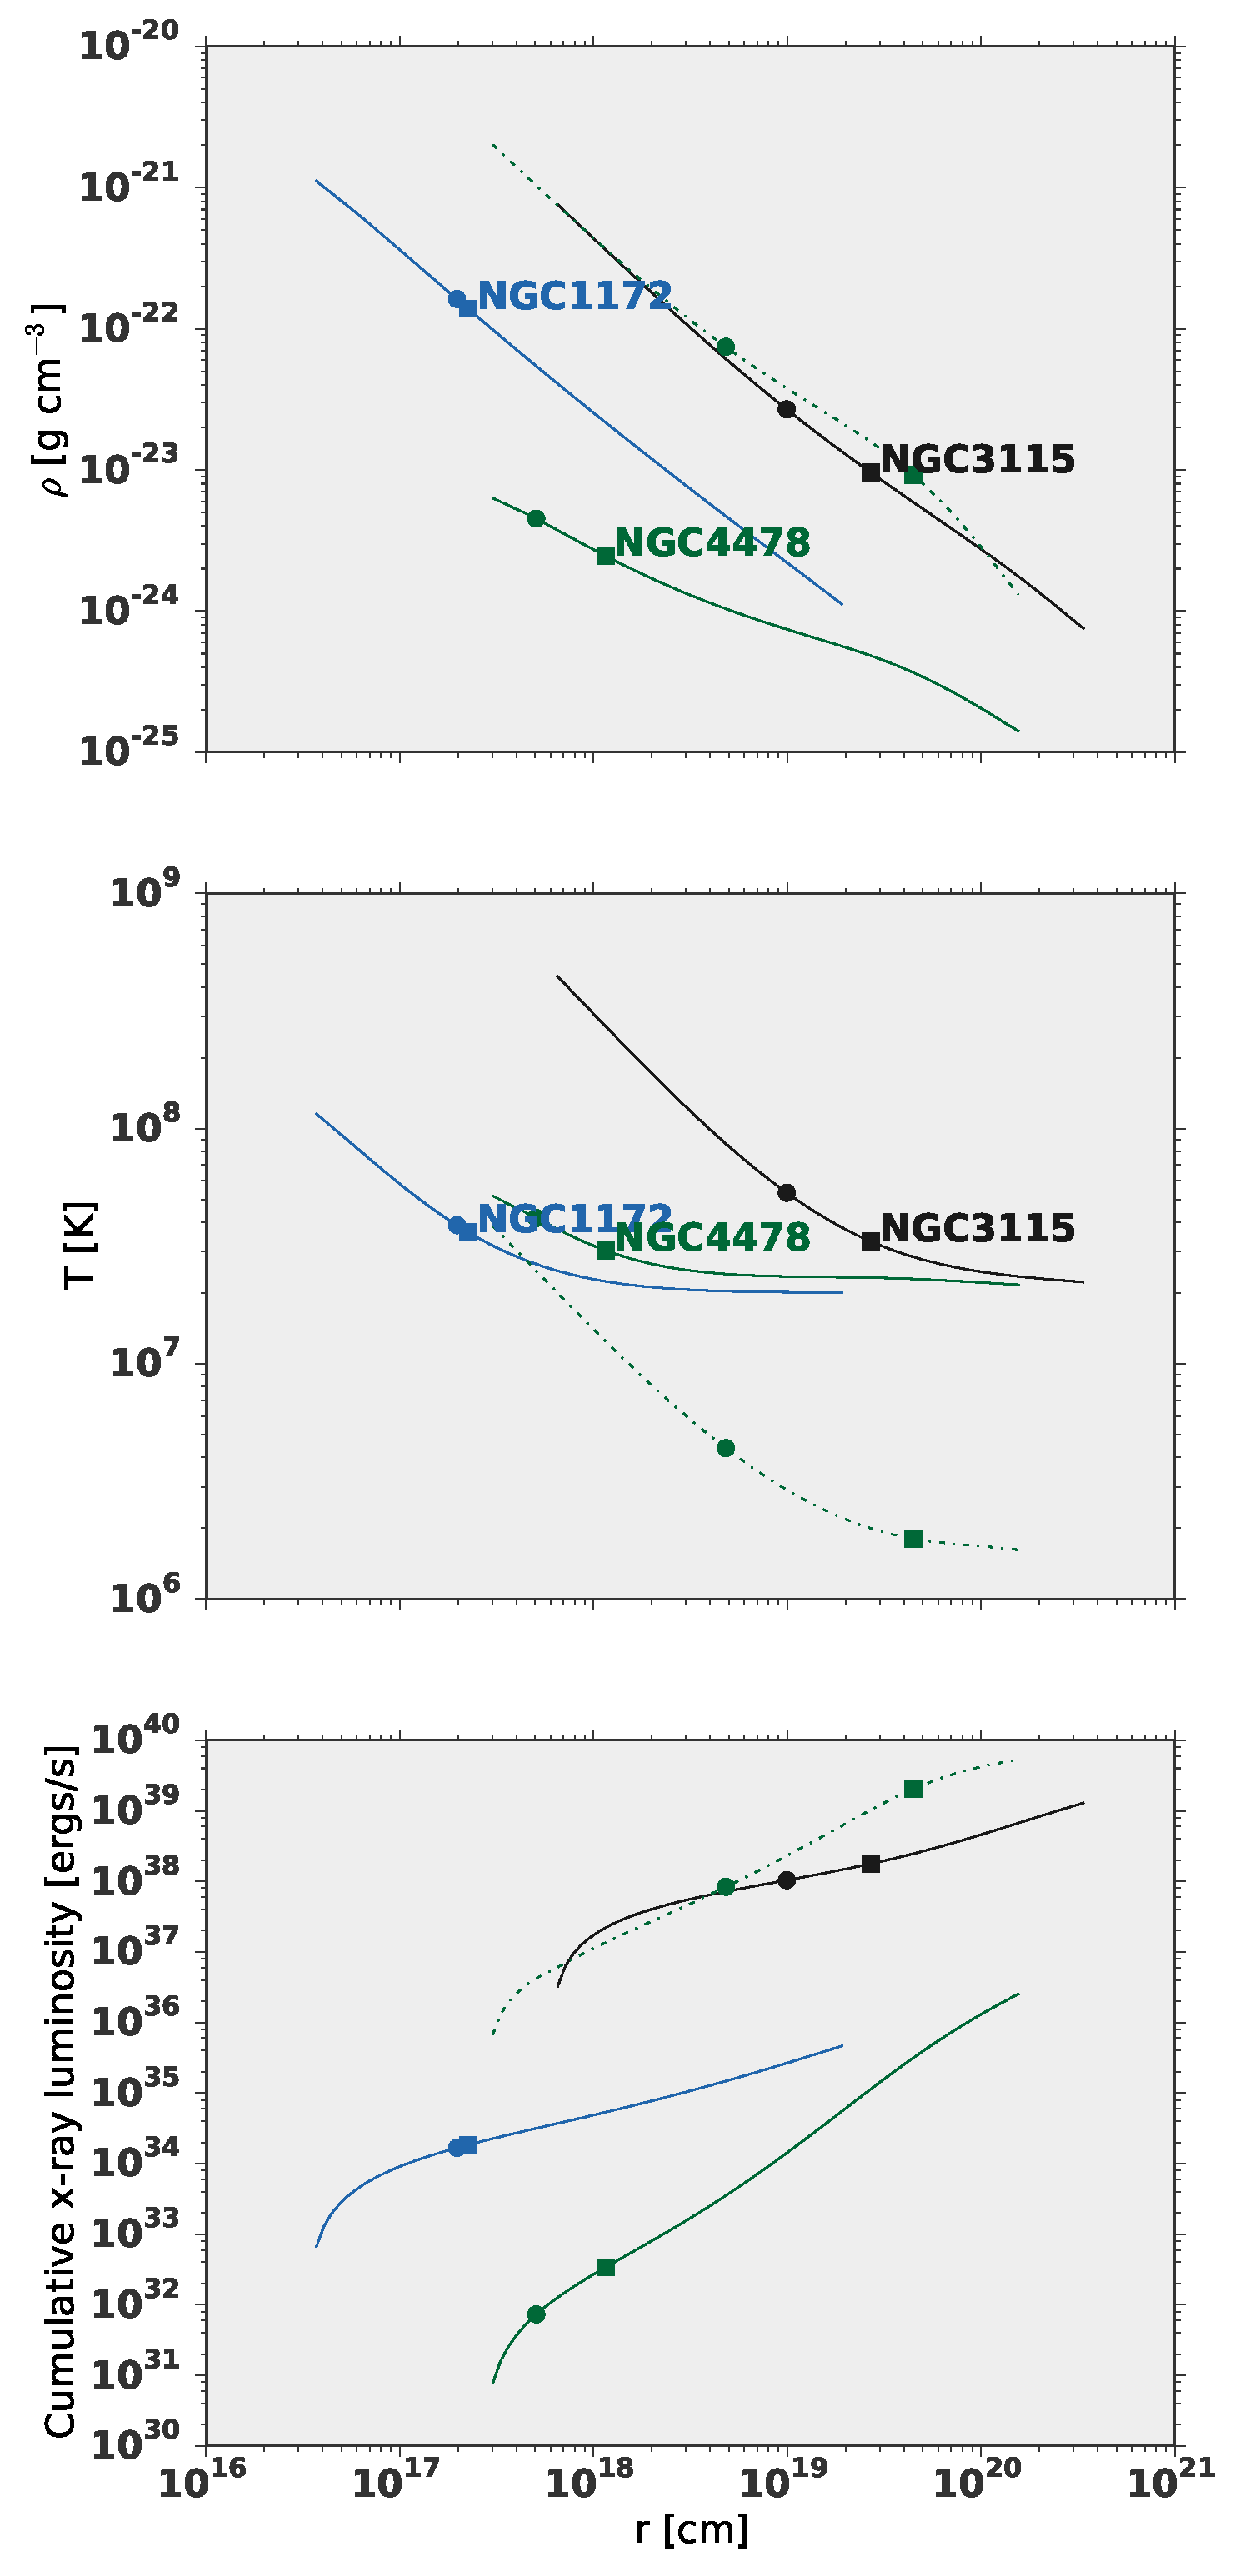
\includegraphics[width=\columnwidth]{profiles.eps}
\caption{\label{fig:profiles}Radial for three different galaxies: NGC1172, NGC4478, and NGC3115. Solid curves correspond to $v_w$=1000 km/s.
The Dot-dashed curve corresponds to $v_w$=200 km/s. Top panel: Density; 
Middle Panel: Temperature; Bottom Panel: X-ray luminosity enclosed within radius $r$.}
\end{figure}

\begin{figure}
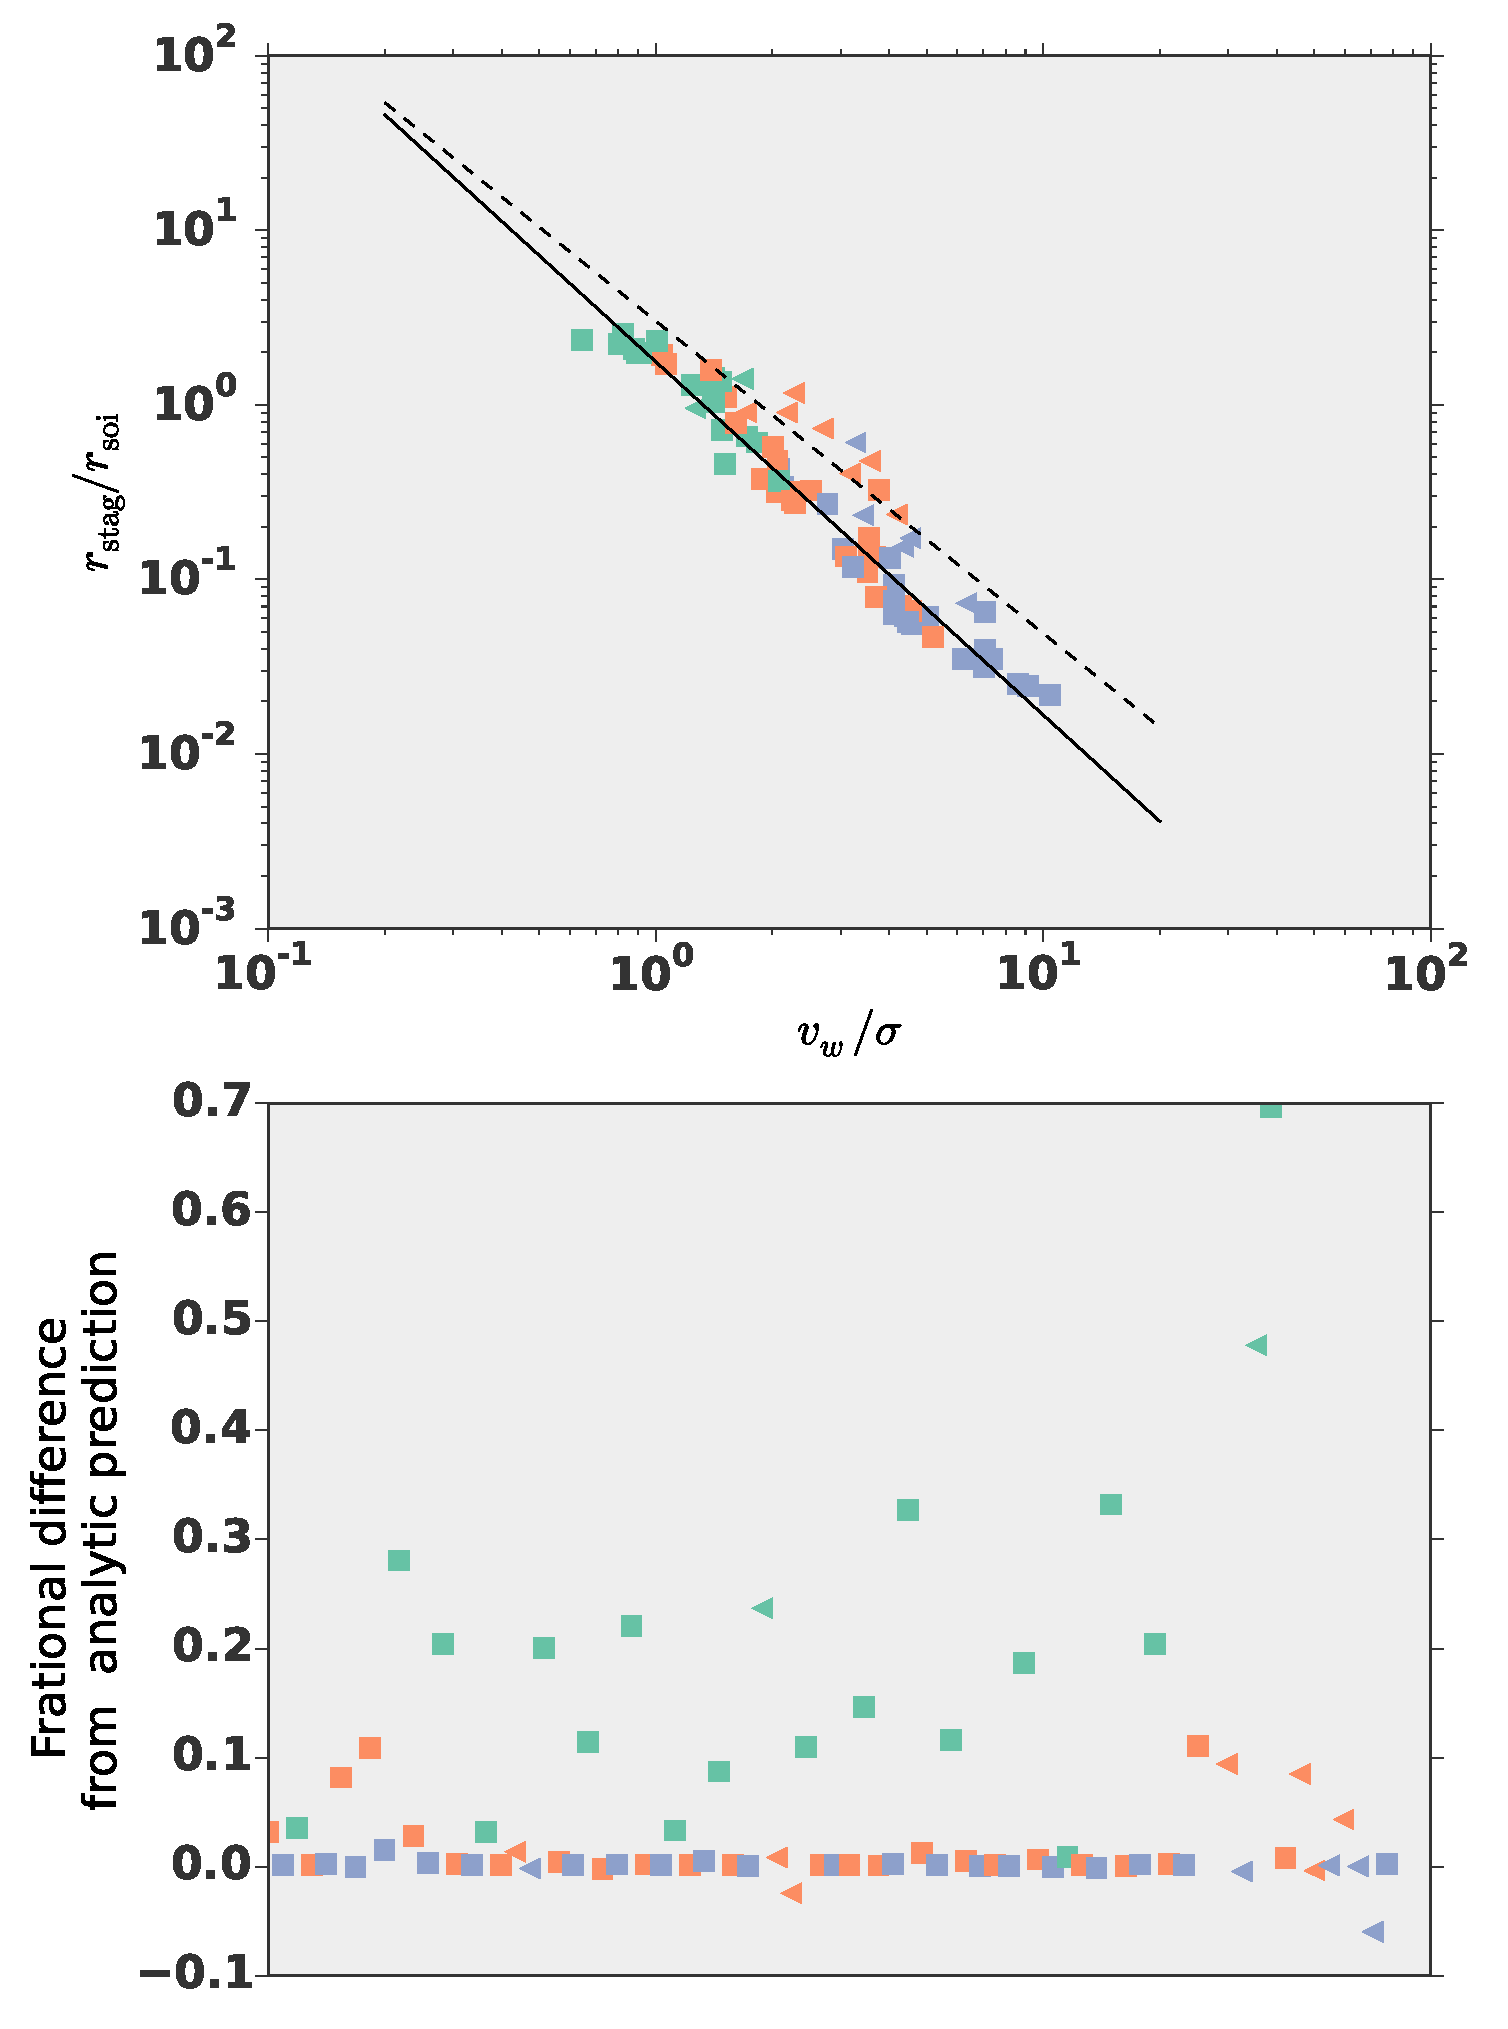
\includegraphics[width=\columnwidth]{rs.eps}
\caption{\label{fig:stag}$\x$ vs. $\vwNorm$}
\end{figure}


\section{Discussion}
\subsection{Heating}
We now discuss potential sources of heating and discuss how different physical sources of heating would lead to different values of $\vwO$. For each heating source  from the specific heating rate $E$ we may estimate the corresponding $\vwO$...

\begin{enumerate}
\item \emph{Stellar winds} The contribution to the heating rate from the red giant winds themselves will be negligible, as red giants have wind velocities $\lsim 40$ km/s.

Although red giant winds dominate the mass budget, winds from main sequence stars may make a significant contribution to the energy budget, with wind velocities $\sim 100-150$ km/s \citep{NaimanSoares-Furtado+:2013a}. 
%%Even assuming efficient thermalization wouldn't the contribution of main sequence winds be diluted by the fraction they take up of the mass budget.

\item \emph{Type Ia SNe} Following \citealt{ShcherbakovWong+:2014a}, the energy injected per Ia SNe is 10$^{51}$ ergs, and the SNe rate is $\simeq 4 \times 10^{-14} \Msun^{-1}$ yr$^{-1}$.  Assuming that each SNe in 10$^{51}$ ergs and a mass injection rate (from stellar winds) of 10$^{-11} \Msun$  yr$^{-1}$, this leads to $\vwO\simeq 600$ km/s.  (Note one of our chosen values for $\vwO$ is 500 km/s).

As noted in \citealt{ShcherbakovWong+:2014a}, it is not obvious whether or not the SNe energy injection treated as a constant throughout time and space, since the flow time-scale may be short compared to the time between successive SNe Ia...
%Thornton and Benton...
\item \emph{MS Pulsars} 
\end{enumerate}

\subsection{Mass accretion rate}
For each of our solutions, we may calculate the accretion rate $\dot{M}$ onto the SMBH. We show $\Medd$ vs. $\Mbh$ as a function of black hole mass for our three  chosen values of the $\vwO$ (200 km/s, 500 km/s, and 1000 km/s). The results are shown in Figure~\ref{fig:mdot_mass}

We find there is a trend of $\eddr$ increasing towards higher black hole masses. However, previous work  suggests a downsizing trend: for quiescent galaxies $L_X \sim \Mbh^\alpha$, where $\alpha\simeq 0.7-0.8$ \citep{Miller+:2013a}. If $L_X\sim\dot{M}^2$, this would suggest $\eddr\sim \Mbh^{-0.6}$. In contrast for fixed $\vwO$ and $\eta$ we obtain that $\eddr\sim \Mbh^{0.5-1}$. One possible solution is that $\eta$ decreases with $\Mbh$. $\dot{M}$ scales linearly with $\eta$, so we would need to have $\eta\sim \Mbh^{-1}$ to explain the observed downsizing trend.  

\begin{figure}
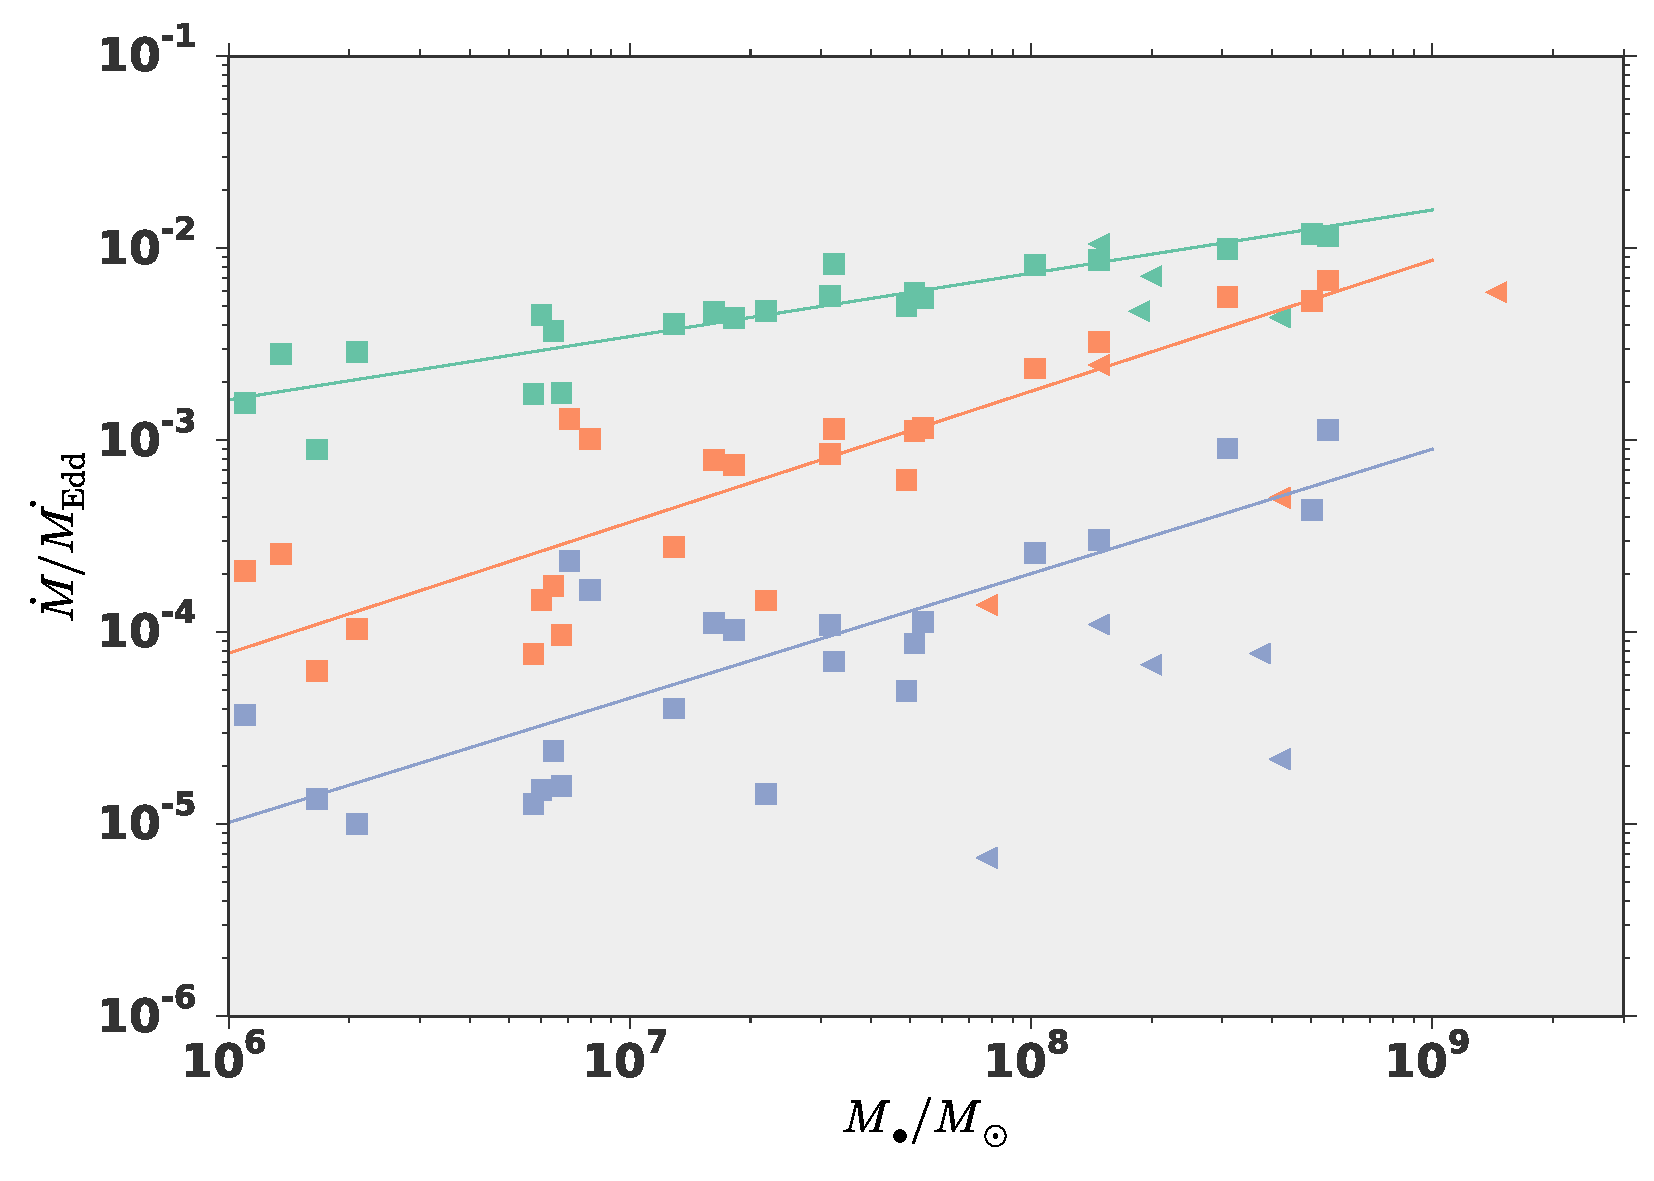
\includegraphics[width=\columnwidth]{mdot_mass.eps}
\caption{\label{fig:mdot_mass}$\eddr$ vs. $\Mbh$}
\end{figure}

%%AG: Split galaxies into cores (squares) and cusps (triangles). For cores only did those galaxies which had all three values of the wind velocity completed. Also want to include a plot of x-ray luminosity (less abstract than the mass accretion rate). 

\subsection{Comparison with observations}
\citealt{AllenDunn+:2006a} use Chandra x-ray observations to infer the temperature and density profiles for nine nearby x-ray luminous elliptical galaxies.  Five of the galaxies in their sample overlap with that in \citetalias{WangMerritt:2004a}. 

We may compare our results for the $T$ and $\rho$ profiles of the overlapping galaxies, with those inferred from observations.  Note that we we have two free parameters ($\eta$ and $\vwO$ in our model and thus we can can always match $T$ and $\rho$ at least one point.  We generally find that $\vwO=500$ km/s (as would be expected from SNe Ia) gives rough agreement with the observed temperatures.  Thus, we choose $\vwO=500$ km/s.  We choose an $\eta$ so that our solution would be consistent with the observed density profiles. The comparison is shown in Figure~\ref{fig:allen_compare}.


\begin{itemize}
\item \emph{NGC4486} On scales of $\sim1$ kpc the density profile in \citealt{AllenDunn+:2006a}  is shallower than in our model. Our model has a break in the gas density at $\sim 300$ pc--near the location of the Nuker break radius for this galaxy at 560 pc. There is an observed break in the density, but on a scale of a few kpc.

In contrast to a naive extrapolation of the observed $T$ and $\rho$ to smaller scales, our models have $T$ and $\rho$ monotonically increasing towards the galactic center. The increase in $T$ is due to the increased velocity dispersion (and thus increased heating) towards the galactic center.
\end{itemize}

\begin{figure*}
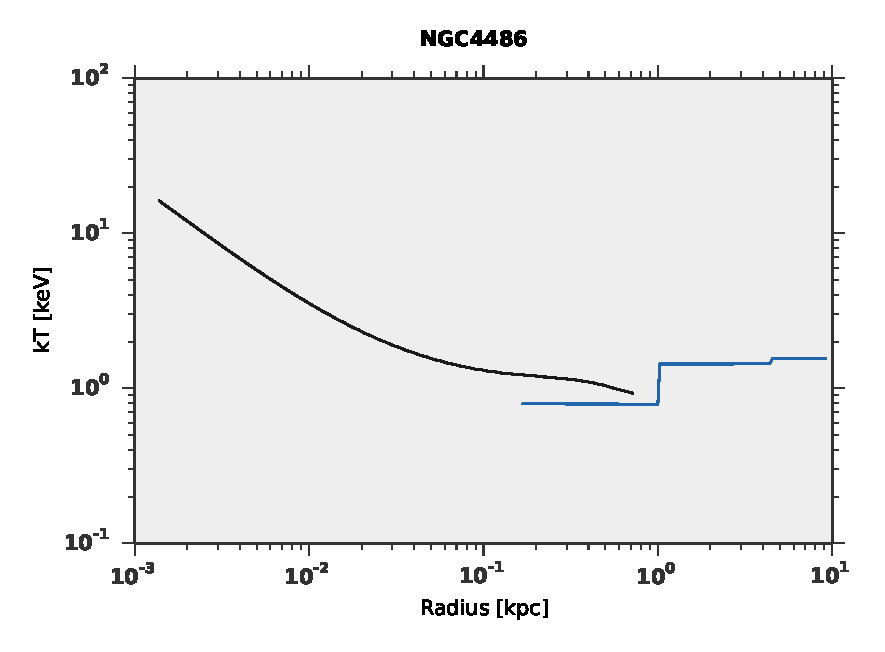
\includegraphics[width=\columnwidth]{T_compare.eps}
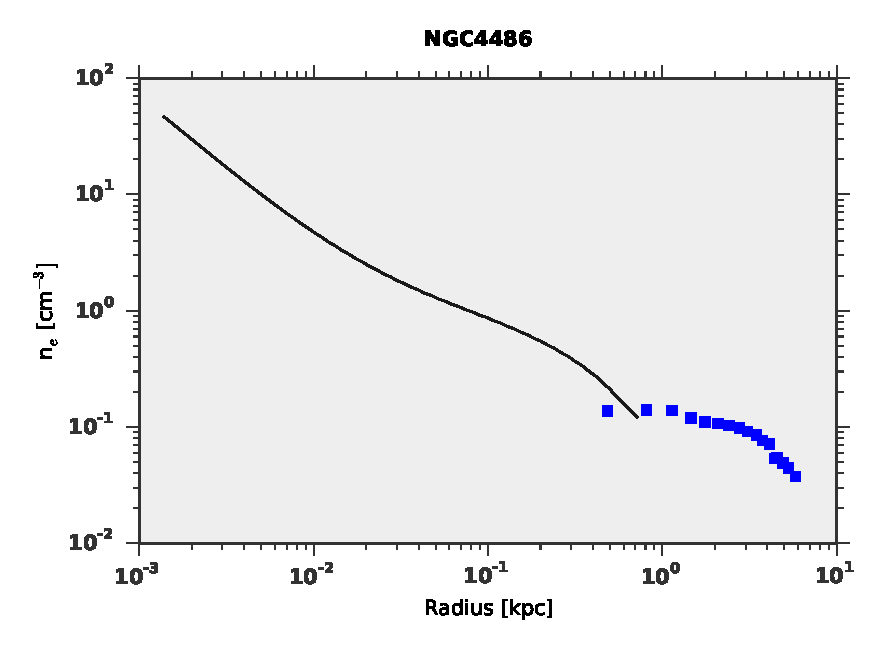
\includegraphics[width=\columnwidth]{dens_compare.eps}
\caption{\label{fig:allen_compare} Comparison to \citealt{AllenDunn+:2006a}}
\end{figure*}


 
\subsection{Cooling}
\label{sec:cooling}

\subsection{Conduction}
\label{sec:conduction}{

\subsection{Angular Momentum}

\section{Summary}


\footnotesize{
  \bibliographystyle{mn2e}
  \bibliography{master}
}
\end{document}
